\documentclass[thmcnt=section, 12pt]{my-elegantbook}

% index page
\usepackage{imakeidx}
\makeindex[columns = 2, intoc, options= -s index_style.ist]

% Title and author
\title{Mathematical Analysis}
\author{Isaac FEI}

\cover{cover}

\begin{document}

% Print title and cover page
\maketitle

% Print table of contents
\frontmatter
\tableofcontents
\mainmatter

%------------------------------
% Main document starts from here
%------------------------------

%==============================
\chapter{Limits and Continuity}

%------------------------------
\section{Limit of a Function}

%------------------------------
\begin{proposition} \label{pro:2}
    Let $f$ and $g$ be complex-valued functions defined on a subset $A$ of a metric space $(X, d)$, and $p$ a limit point of $A$. If $\lim_{x \to p} f(x) = 0$ and $g$ is bounded, then 
    \begin{align*}
        \lim_{x \to p} f(x)g(x) = 0
    \end{align*}
\end{proposition}

\begin{proof}
    % TODO
\end{proof}

%------------------------------

\section{Continuous Functions}

%------------------------------

The next theorem states that the composite function of continuous functions is also continuous.

\begin{theorem} \label{thm:3}
    Let $(X, d_X)$, $(Y, d_Y)$ and $(Z, d_Z)$ be metric spaces. Let $f: X \to Y$ and $g: Y \to Z$ be functions, and let $h = g \circ f$ be the composite function defined on $X$. If $f$ is continuous at $p \in X$, and $g$ is continuous at $f(p)$, then $h$ is continuous at $p$.
\end{theorem}

\begin{proof}
    Given $\varepsilon > 0$, since $g$ is continuous at $f(p)$, there exists some $\delta^\prime > 0$ such that
    \begin{align}
        d_Y(y, f(p)) < \delta^\prime
        \implies d_Z(g(y), g(f(p))) < \varepsilon
        \label{eq:7}
    \end{align}
    And since $f$ is continuous at $p$, there exists some $\delta > 0$ such that 
    \begin{align}
        d_X(x, p) < \delta
        \implies d_Y(f(x), f(p)) < \delta^\prime
        \label{eq:8}
    \end{align}
    Now, choosing $x \in X$ satisfying $d_X(x, p) < \delta$, and then applying \eqref{eq:8} followed by \eqref{eq:7}, we have
    \begin{align*}
        d_Z(g(f(x)), g(f(p))) < \varepsilon
    \end{align*} 
    This is precisely $d_Z(h(x), h(p)) < \varepsilon$. Hence, $h$ is continuous at $p$.
\end{proof}

%------------------------------

\begin{theorem} \label{thm:6}
    Let $f: X \to \R$ be a real-valued function from a metric space $X$ to $\R$. Let $K \subset X$ be a compact subset. Then there exist points $p, q \in K$ such that 
    \begin{align*}
        f(p) = \sup f(K)
        \quad \text{and} \quad
        f(q) = \inf f(K)
    \end{align*}
\end{theorem}

%==============================

\chapter{Differentiation}

Let our exploration begins with real-valued functions defined on real numbers.

%------------------------------

\section{Definition of Derivative}

Observe the slopes of secant lines (displayed as dashed lines) of the curve shown in Figure~\ref{fig:1}

\begin{figure}[H]
    \centering
    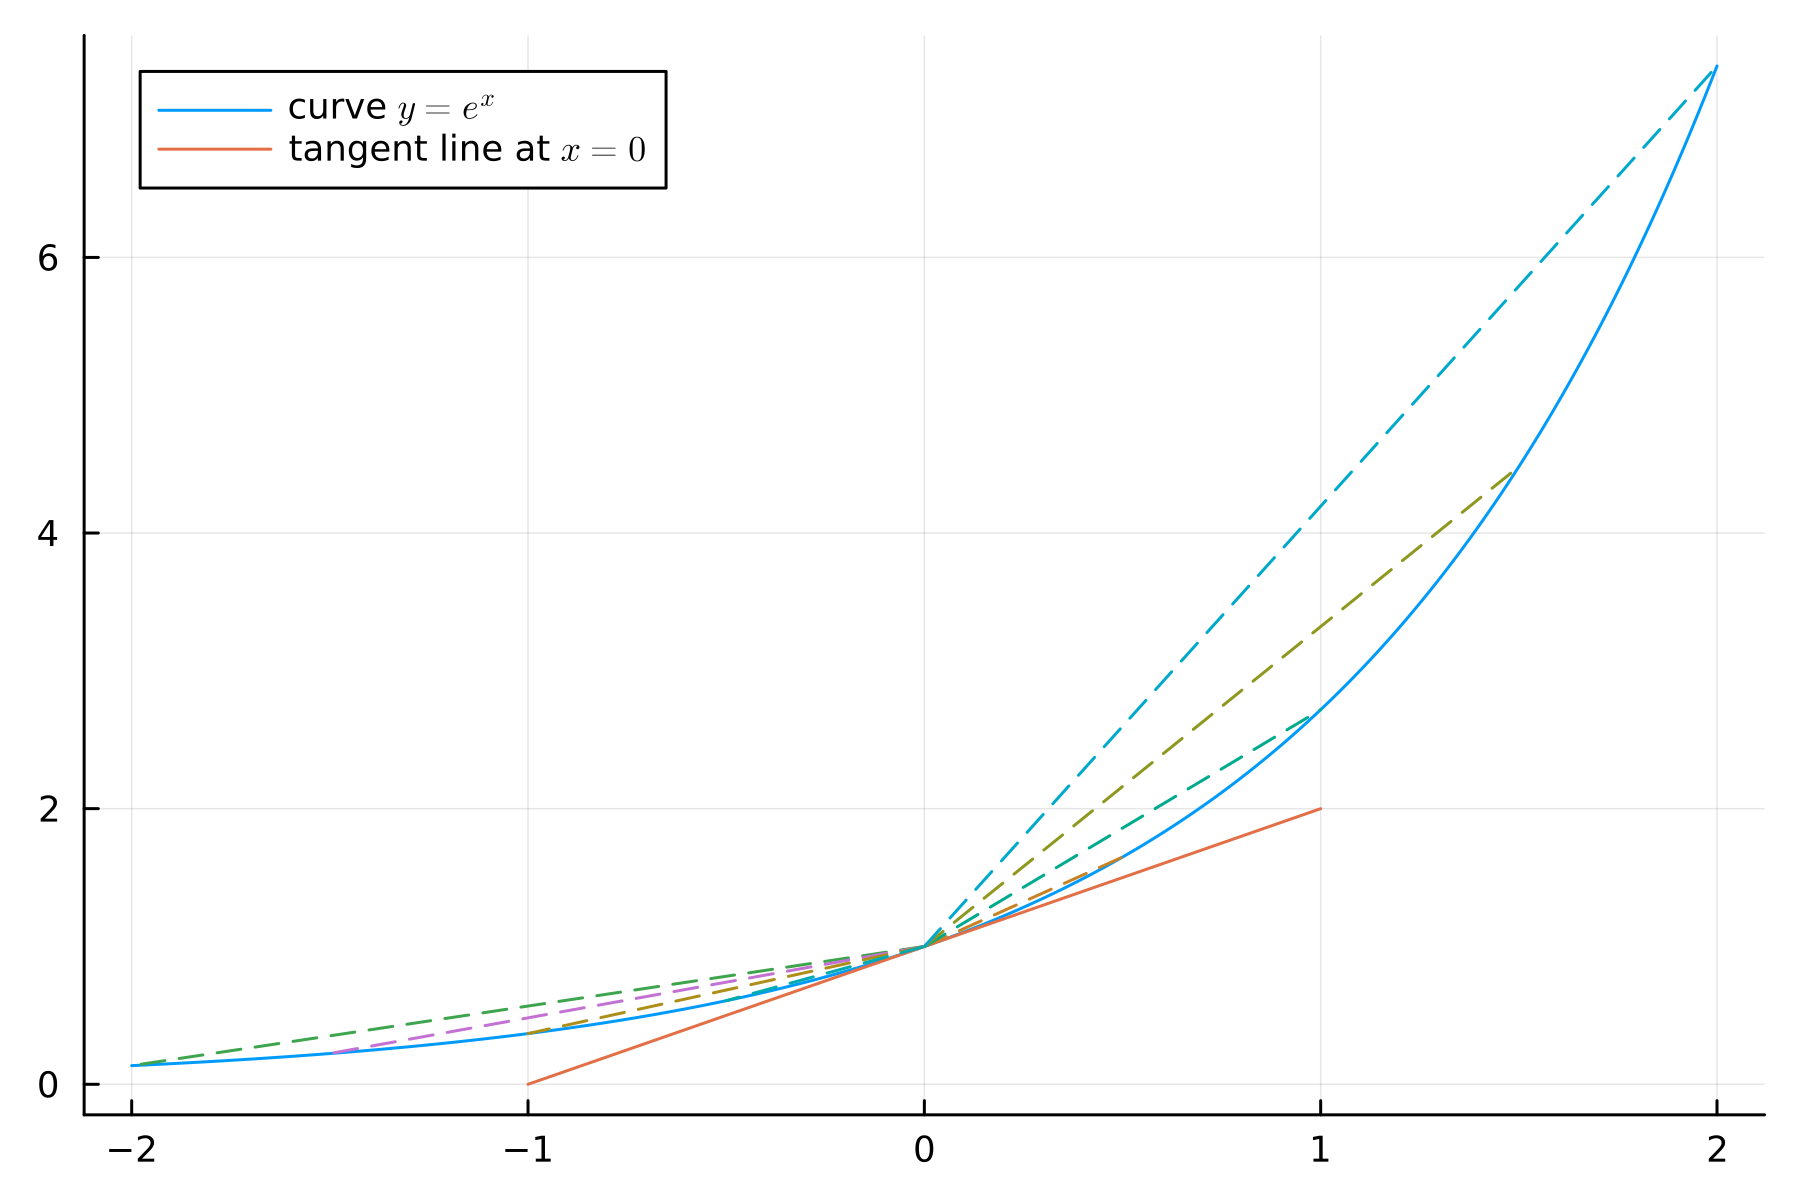
\includegraphics[scale=0.2]{figures/secant-lines-and-a-tangent-line.png}
    \caption{Secant lines and a tangent line of curve $y=e^x$.}
    \label{fig:1}
\end{figure}

\noindent All secant lines have a common point of intersection, $(0, 1)$. And as the other intersection point gets closer and closer to $(0, 1)$, the slope of the secant line tends to converge to some number. This number, the limiting slope, is precisely the \textbf{derivative} of this curve/function at $x=0$, which we shall soon define. We can draw a straight line passing through the point $(0,1)$ with the limiting slope. This line is then called the tangent of the curve at point $(0,1)$, as illustrated in Figure~\ref{fig:1}. 

\begin{definition}
    Let $f$ be defined on an open interval $(a, b)$, and let $c \in (a, b)$ an interior point. Then $f$ is said to be \textbf{differentiable}\index{differentiable functions} at $c$ if the limit 
    \begin{align*}
        \lim_{x \to c} \frac{f(x) - f(c)}{x - c}        
    \end{align*}
    exists. This limit, denoted by $f^\prime(c)$, is called the \textbf{derivative} \index{derivative} of $f$ at point $c$.
\end{definition}

If $f^\prime(c)$ exists $\forall c \in I$ for some interval $I$, then we can define a function $f^\prime$ on $I$, which is called the derivative of $f$. Here the word \textit{derivative} means a function instead of just a number. 

%------------------------------

The definition of derivatives we present here involves the limit obtained by letting one point approach the other one, $x \to c$. For computational convenience, we can treat the derivative of $f$ at $c$ as the limit of the fraction $[ f(c+h) - f(c) ] / h$ as $h \to 0$. That is, the limit is reached when the distance between points $x$ and $c$, $h = \abs{x-c}$, is small. The following proposition states this idea formally.

\begin{proposition} \label{pro:1}
    Let $f$ be defined on $(a, b)$. Then $f$ is differentiable at $c \in (a, b)$ if and only if 
    \begin{align}
        \lim_{h \to 0} \frac{f(c+h) - f(c)}{h} 
        \label{eq:3}
    \end{align}
    exists. In that case, $f^\prime(c) = \lim_{h \to 0} [ f(c+h) - f(c) ] / h$.
\end{proposition}

\begin{proof}
    Suppose $f$ is differentiable at $c$. For an arbitrary $\varepsilon > 0$, there exists $\delta > 0$ such that 
    \begin{align*}
        \abs{x - c} < \delta
        \implies \abs{\frac{f(x) - f(c)}{x - c} - f^\prime(c)} < \varepsilon
    \end{align*}
    Let number $h$ be such that $\abs{h} < \delta$. Then since $\abs{(c+h) - c} = \abs{h} < \delta$, we have 
    \begin{align*}
        \abs{\frac{f(c+h) - f(h)}{h} - f^\prime(c)}
        = \abs{\frac{f(c+h) - f(h)}{(c+h) - c} - f^\prime(c)} < \varepsilon
    \end{align*}
    This implies the limit \eqref{eq:3} exists, and it equals $f^\prime(c)$.

    Conversely, suppose the limit \eqref{eq:3} exists, say it equals $L$. Then for $\varepsilon > 0$ there exists $\delta > 0$ such that 
    \begin{align*}
        \abs{h} < \delta
        \implies \abs{\frac{f(c+h) - f(c)}{h} - L} < \varepsilon
    \end{align*}
    Choose $x$ such that $\abs{x - c} < \delta$, we have 
    \begin{align*}
        \abs{
            \frac{f(x) - f(c)}{x - c} - L
        } = \abs{
            \frac{f(c + (x - c)) - f(c)}{x - c} - L
        } < \varepsilon
    \end{align*}
    Therefore, the limit $[f(x) - f(c)]/(x - c)$ exists, which is equal to $L$. By the definition of derivatives, $f$ is differentiable at $c$, and $f^\prime(c) = L$.
\end{proof}

\begin{exercise}
    Calculate the derivative of $e^x$ at $x = 0$. 

    \noindent [Hint: You may use the fact $e^x = \sum_{n=0}^\infty \frac{x^n}{n!} =  1 + x + \frac{1}{2} x^2 + \frac{1}{6} x^3 + \cdots$.]
\end{exercise}

\begin{exercise}
    Calculate the derivative of
    \begin{align*}
        f(x) 
        = x^2 \sin \frac{1}{x^2} \ind\{x \neq 0\}
        = \begin{cases}
            x^2 \sin \frac{1}{x^2} &x \neq 0 \\ 
            0 &x=0
        \end{cases}
    \end{align*}
    at $x = 0$.
    \label{ex:1}
\end{exercise}

\begin{solution}
    We have 
    \begin{align*}
        \frac{f(0+h) - f(0)}{h}
        = h \sin \frac{1}{h^2}
    \end{align*}
    Note the limit of the above expression is zero as $h \to 0$ by Proposition~\ref{pro:2} since $\lim_{h\to 0} h = 0$ and $\sin (1/h^2)$ is bounded by $1$. Hence, $f^\prime(0) = 0$ by Proposition~\ref{pro:1}.

    The graph of $f(x)$ is shown in Figure~\ref{fig:2}. As we can see, $f(x)$ is clamped between curves $y=x^2$ and $y=-x^2$ with the same tangents $y=0$ at $x=0$. And we have shown $f^\prime(0)=0$, which means that the tangent of $f(x)$ is also $y=0$ at $x=0$. What conjecture can you make?

    \begin{figure}[ht]
        \centering
        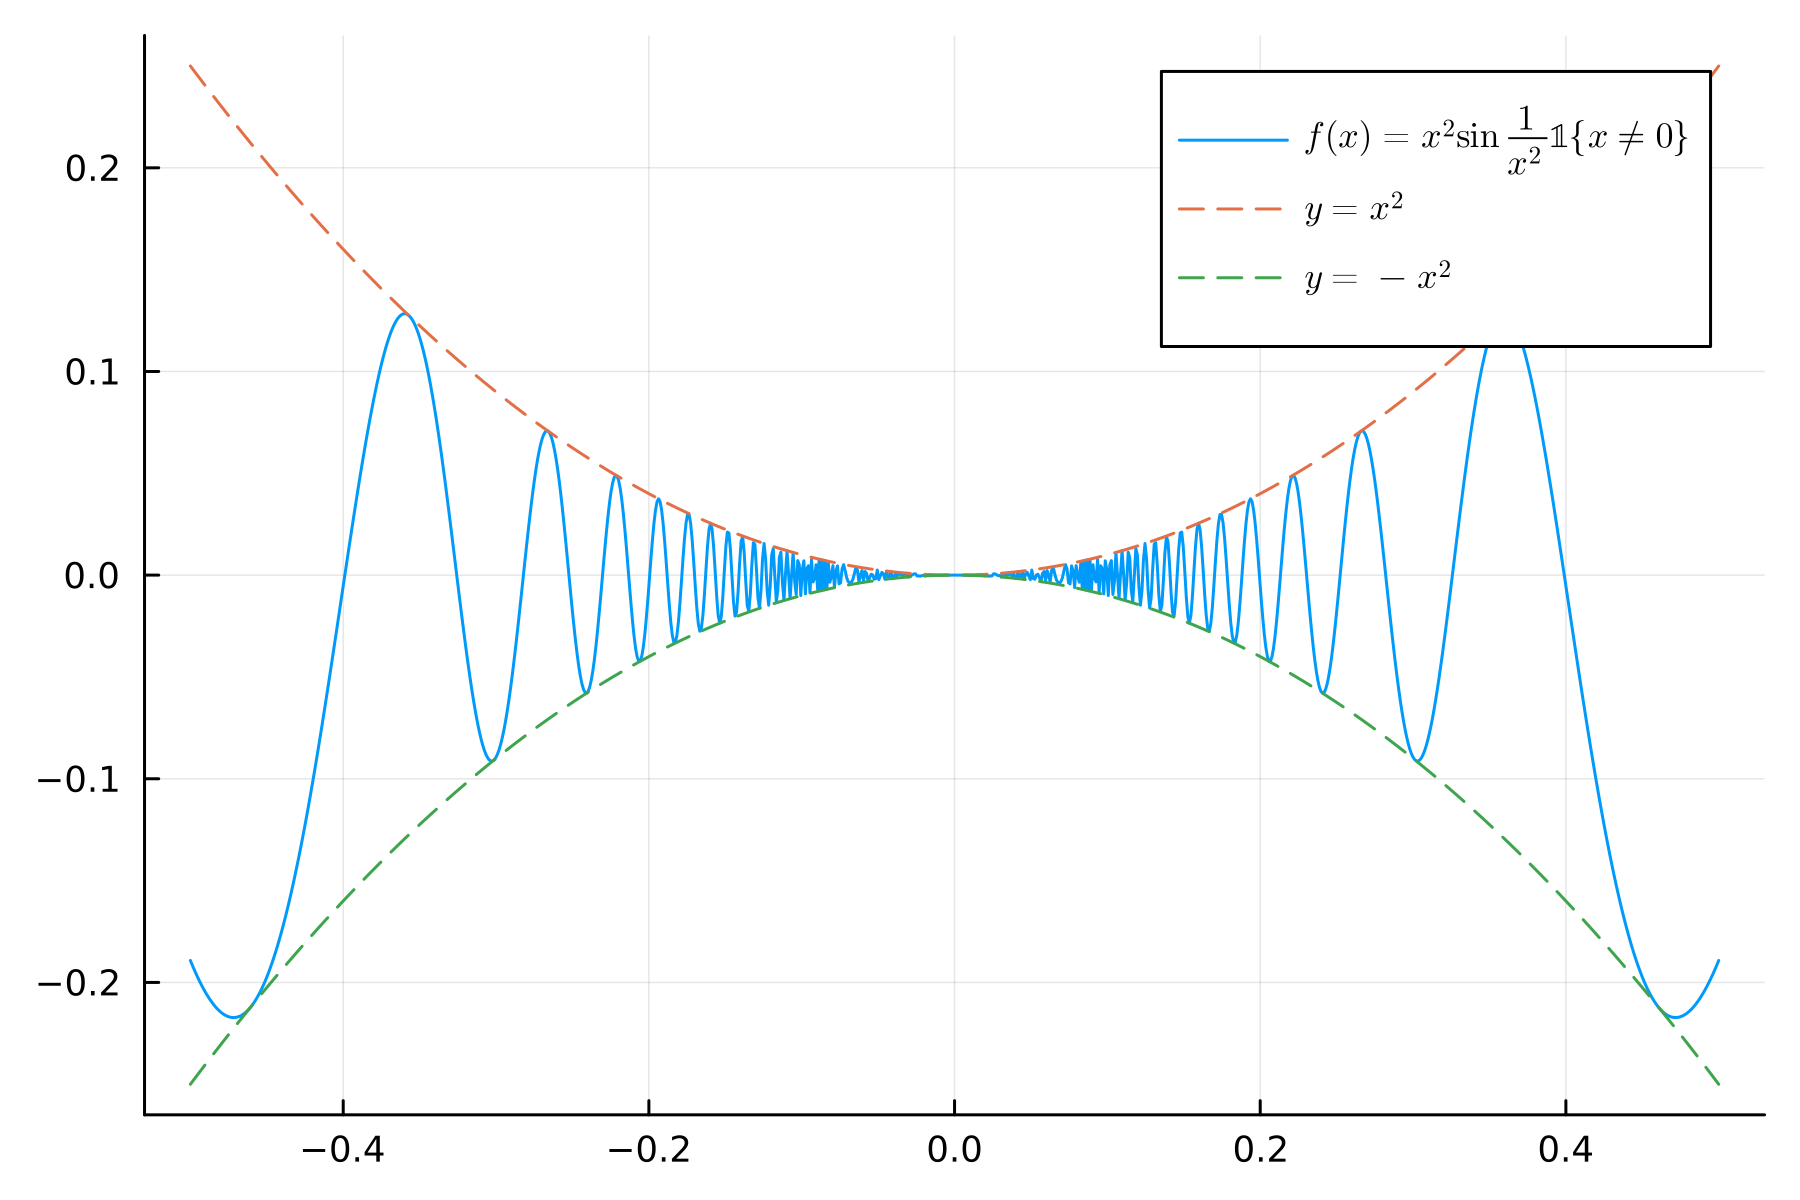
\includegraphics[scale=0.2]{figures/graph-001.png}
        \caption{Graph of $f(x) = x^2 \sin \frac{1}{x^2} \ind\{x \neq 0\}$.}
        \label{fig:2}
    \end{figure}

    Moreover, we observe that $f(x)$ crosses its tangent line at $x=0$ infinitely many times. This example shows that the tangent line does not have to touch the curve only at one point.
\end{solution}

%------------------------------

\subsection{One-Sided Derivatives and Infinite Derivatives}

So far, the point at which the derivative is defined has to be an \textit{interior} point. Sometimes, we are required to consider the derivatives at the endpoints of the interval. For example, as we shall see in more detail in Chapter~\ref{chap:1}, we need to take the derivative of function $F(x) = \int_a^x f(t) \mathrm{d}t$ at $x=a$. Hence, we are motivated to define the \textbf{one-sided derivatives}\index{one-sided derivatives}. 

If we consider the derivative of $f$, $f^\prime$ as a function, then $f^\prime(x)$ may tend to infinity as $x$ approaches an endpoint. In addition, sometimes we need to interpret the meaning of vertical tangent lines. This leads to the definition of \textbf{infinite derivatives}\index{infinite derivative}.

\begin{definition}
    Let $f$ be defined on a closed interval $I$. Suppose $f$ is continuous at point $c \in I$. Then $f$ is said to have a \textbf{right-hand derivative}\index{right-hand derivative} at $c$ if the right-hand limit 
    \begin{align*}
        \lim_{x \to c^{+}} \frac{f(x) - f(c)}{x - c}
    \end{align*}
    exists as a finite number, or the limit is $\infty$ or $-\infty$. This right-hand derivative shall be denoted by $f^\prime_{+}(c)$. The \textbf{left-hand derivative}\index{left-hand derivative}, denoted by $f^\prime_{-}(c)$, is defined similarly. In addition, if $c$ is an interior point, and $f^\prime_{+}(c) = f^\prime_{-}(c) = \infty$, then we write $f^\prime(c) = \infty$. $f^\prime(c) = -\infty$ is similarly defined.
\end{definition}

\begin{remark}
    Note that though we write $f^\prime(c) = \infty$ or $f^\prime(c) = -\infty$, we do not say $f$ is differentiable there.
\end{remark}

It is not very intuitive to imagine, at first thought, a continuous function having infinite derivatives. But there are quite a lot of such examples.

\begin{example}
    The first example is constructed by cutting a circle in the middle. If we cut a circle in half and stick the lower half to the right of the upper one, then we have a function with a vertical tangent line in the middle. The explicit expression of this function is 
    \begin{align*}
        f(x) = \begin{cases}
            \sqrt{1 - (x-1)^2} &0 \leq x \leq 2 \\ 
            - \sqrt{1 - (x-3)^2} &2 < x \leq 4
        \end{cases}
    \end{align*}

    \begin{figure}[ht]
        \centering
        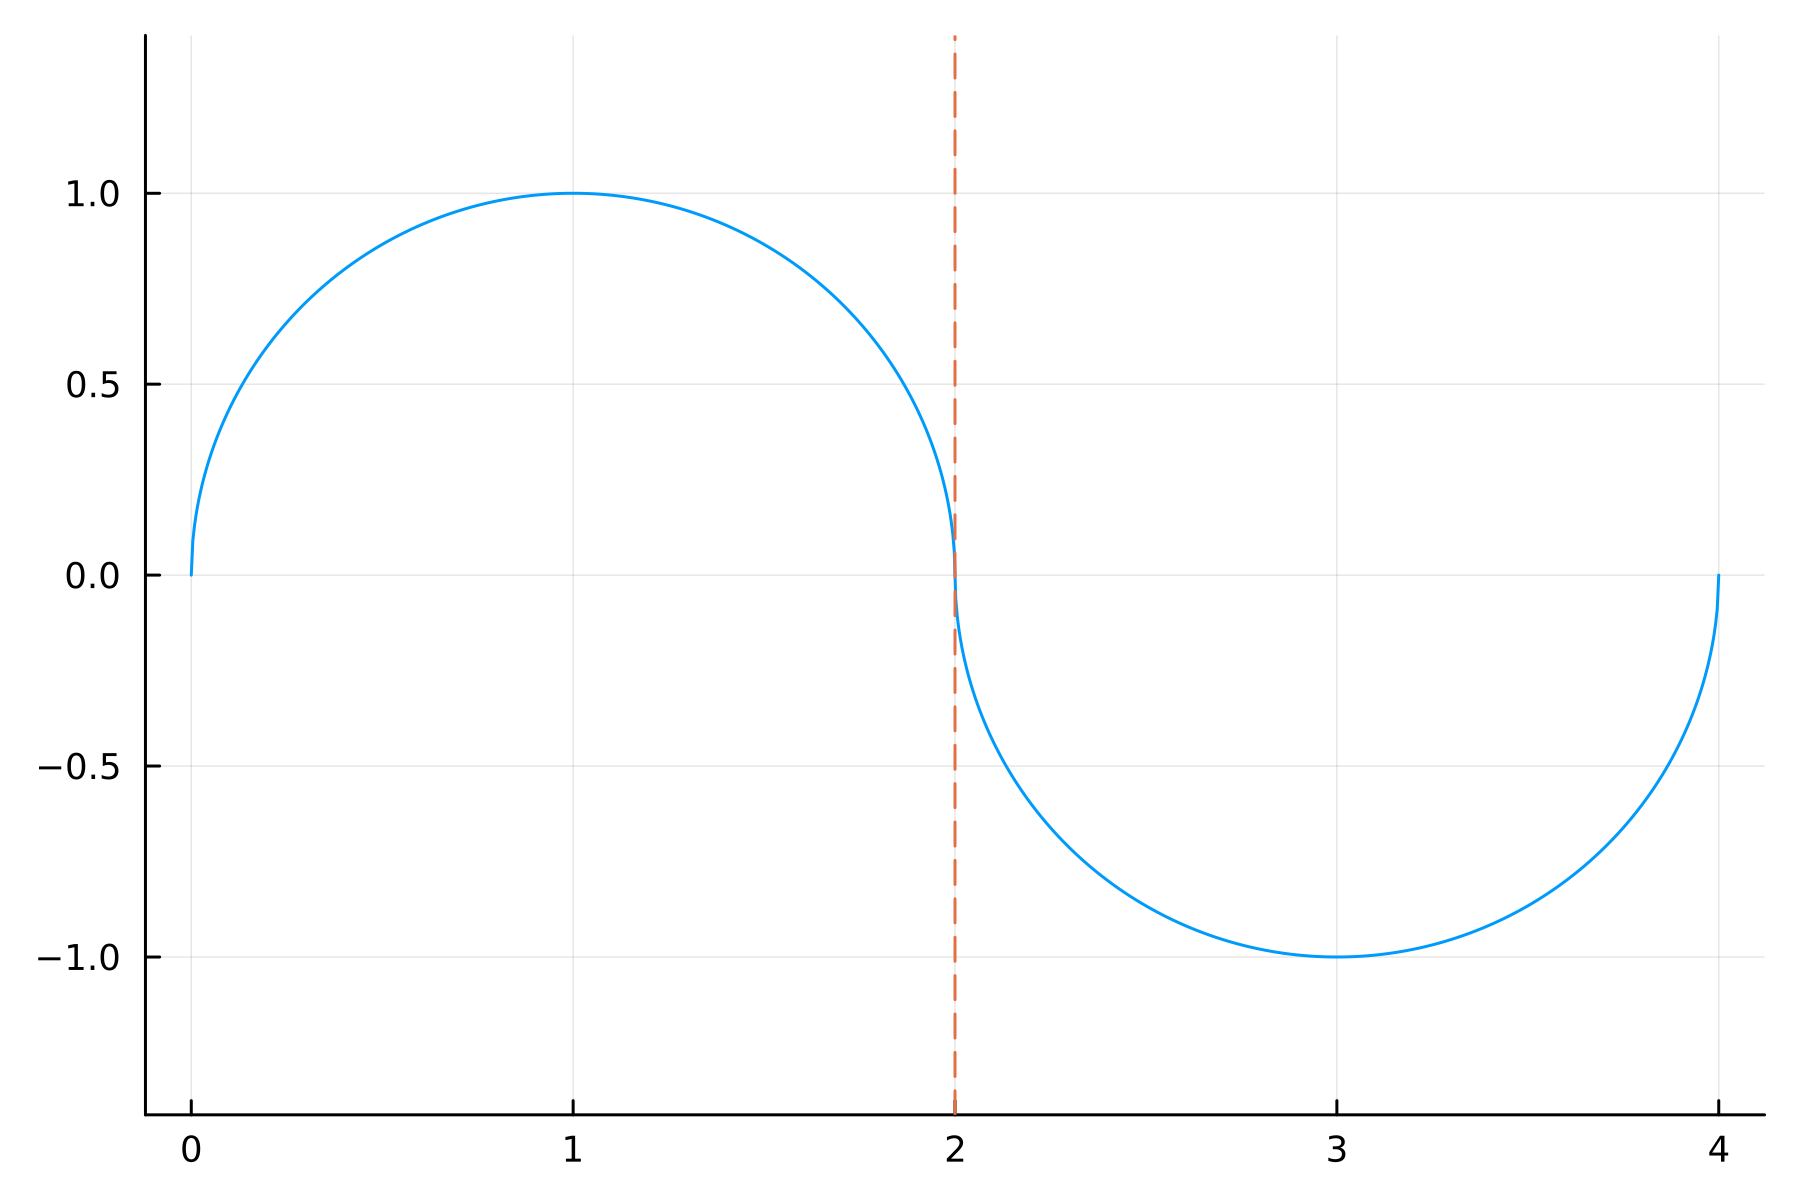
\includegraphics[scale=0.2]{figures/graph-002.png}
        \caption{Graph of $f(x) = \sqrt{1-(x-1)^2}\ind\{0 \leq x \leq 2\} - \sqrt{1-(x-3)^2}\ind\{2 < x \leq 4\}$.}
    \end{figure}

    \noindent The function is continuous and one can show that $f^\prime(2) = -\infty$.
    \label{eg:1}
\end{example}

\begin{example}
    The following next example includes both positive and negative intuitive derivatives, and a point at which the right and left-hand side derivatives are $\infty$ and $-\infty$, respectively. Consider the function 
    \begin{align*}
        f(x) = \sqrt[3]{x^2 (x-1) (x-2)}
    \end{align*}
    Its graph is shown in Figure~\ref{fig:3}.

    \begin{figure}[ht]
        \centering
        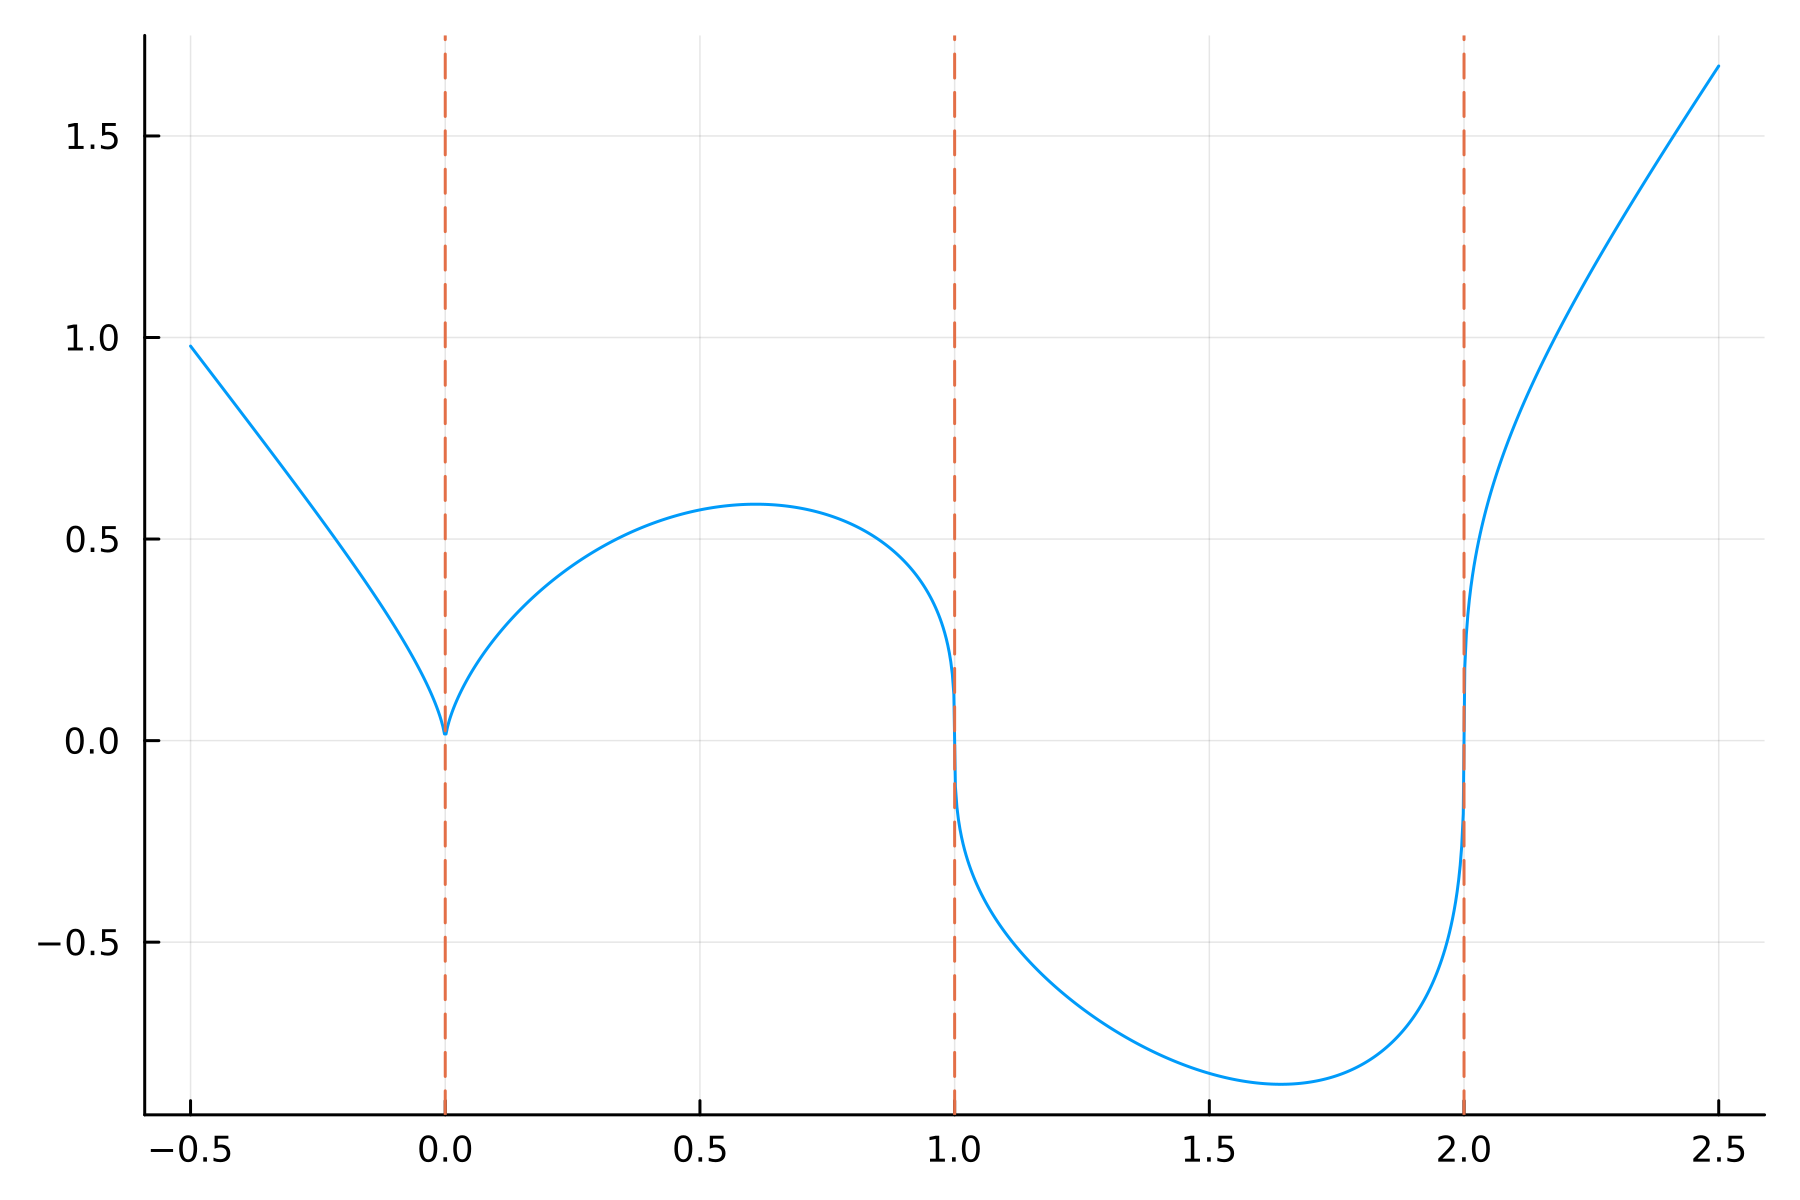
\includegraphics[scale=0.2]{figures/graph-003.png}
        \caption{Graph of $f(x) = \sqrt[3]{x^2 (x-1) (x-2)}$.}
        \label{fig:3}
    \end{figure}    

    It is an exercise to show $f^\prime(1) = -\infty$ and $f^\prime(2) = \infty$. We now consider the one-sided derivatives at $x = 0$. We have 
    \begin{align*}
        \frac{f(x) - f(0)}{x - 0}
        = \sqrt[3]{\frac{(x-1)(x-2)}{x}}
    \end{align*}
    Letting $x \to 0^{+}$ leads to $f^\prime_{+}(0) = \infty$, while $x \to 0^{-}$ yields $f^\prime_{-}(0) = -\infty$. Hence, we say the derivative of $f$ does not exist at $x = 0$.
    \label{eg:2}
\end{example}

%------------------------------

\section{Derivatives and Continuity}

The next theorem helps to reduce some theorems on derivatives to theorems on continuity.

\begin{theorem} \label{thm:1}
    Let $f$ be a function defined on $(a, b)$, and $c \in (a, b)$ a fixed point in that interval. We have the following statements:
    \begin{enumerate}
        \item If $f$ is differentiable at $c$, then there exists a function $\phi$ on $(a, b)$ which is continuous at $c$, and satisfies 
        \begin{align}
            f(x) - f(c) = (x - c) \phi(x)
            \quad \forall x \in (a, b)
            \label{eq:1}
        \end{align}
        And $f^\prime(c) = \phi(c)$.
        \item Conversely, if there exists a function $\phi$ on $(a, b)$ which is continuous at $c$, and satisfies \eqref{eq:1}, then $f$ is differentiable at $c$ with $f^\prime(c) = \phi(c)$.
    \end{enumerate}
\end{theorem}

The function $\phi$ is precisely the slope of function $f$'s secant line.

\begin{proof}
    (Proof of 1) Suppose $f$ is differentiable at $c$. Define 
    \begin{align*}
        \phi(x) = \frac{f(x) - f(c)}{x - c}, 
        \quad x \neq c
        \quad\text{and}\quad 
        \phi(c) = \lim_{x \to c} \frac{f(x) - f(c)}{x - c}
    \end{align*}
    Note that $\phi(c)$ is well-defined since the limit (which equals $f^\prime(c)$) indeed exists by the definition of the derivative of $f$ at $c$. Notice also that by defining function $\phi$ in this way, it is automatically continuous at $c$. And of course, the equation \eqref{eq:1} holds.

    (Proof of 2) It follows from \eqref{eq:1} that 
    \begin{align*}
        \phi(x) = \frac{f(x) - f(c)}{x - c}
        \quad \forall x \neq c
    \end{align*}
    Since $\phi$ is continuous at $c$, by sending $x \to c$, we have 
    \begin{align*}
        \phi(c) = \lim_{x \to c} \phi(x)
        = \lim_{x \to c} \frac{f(x) - f(c)}{x - c}
    \end{align*}
    This implies $f$ is differentiable at $c$, and $f^\prime(c) = \phi(c)$.
\end{proof}

%------------------------------

With the help of Theorem~\ref{thm:1}, we can easily show that $f$ must be continuous at $c$ if it is differentiable there.

\begin{theorem} \label{thm:2}
    Let $f$ be defined on $(a, b)$. If $f$ is differentiable at $c \in (a, b)$, then it is continuous at $c$.
\end{theorem}

\begin{proof}
    By Theorem~\ref{thm:1}, there exists a function $\phi$ on $(a, b)$ such that $\phi$ is continuous at $c$, and
    \begin{align}
        f(x) - f(c) = (x - c) \phi(x)
        \quad \forall x \in (a, b)
        \label{eq:2}
    \end{align}
    Since the limit of the right-hand side in \eqref{eq:2} exists as $x \to c$, the limit of the left-hand side also exists, and 
    \begin{align*}
        \lim_{x \to c} f(x) - f(c)
        = \lim_{x \to c}(x - c) \phi(x)
        = 0
    \end{align*}
    This implies 
    \begin{align*}
        \lim_{x \to c} f(x) = f(c)
    \end{align*}
    Hence, $f$ is continuous at $c$.
\end{proof}

%------------------------------

\section{Computing Derivatives}

It is difficult in practice to compute the derivative of any function only using the definition. In this section, we shall introduce some theorems and standard rules that are helpful with computation. If one knows the derivatives of elementary functions (e.g., $x^a$, $e^x$, $\ln x$, $\sin x$, $\cos x$, etc.), then by applying these theorems, one should be able to compute the derivatives of any functions that are built up out of elementary functions using summations, differences, products, quotients, and compositions.

\begin{note}
    In fact, these so-called elementary functions are not elementary at all. We shall present their definitions as well as their derivatives rigorously in later chapters.
\end{note}

%------------------------------

\subsection{Algebra of Derivatives}

%------------------------------

\begin{theorem}
    Suppose $f$ and $g$ are defined on $(a, b)$ and are both differentiable at $c \in (a, b)$. Then the functions $f + g$, $f - g$, $fg$ are also differentiable at $c$. If $g(c) \neq 0$, then the quotient $f / g$ is also differentiable at $c$. And the formulas of their derivatives are given by 
    \begin{enumerate}
        \item $(f \pm g)^\prime(c) = f^\prime(c) \pm g^\prime(c)$, 
        \item $(f g)^\prime(c) = f^\prime(c) g(c) + f(c) g^\prime(c)$, 
        \item $(f / g)^\prime(c) = \frac{f^\prime(c) g(c) - f(c) g^\prime(c)}{ g^2(c) }$, provided $g(c) \neq 0$.
    \end{enumerate}
\end{theorem}

\begin{remark}
    One might be worried about the possibility that the quotient $f / g$ may only be defined at point $c$ if we only require $g(c) \neq 0$. Then how can we say $f / g$ is differentiable at some point? However, the condition that $g$ is differentiable at $c$ implicitly implies that $g(x) \neq 0$ for $x$ in some interval about $c$ if we assume $g(c) \neq 0$. Take a few seconds and think about why this is true. Note that $g$ is continuous at $c$ by Theorem~\ref{thm:2}. Then, if $g(c) \neq 0$, by the continuity, $g$ is also nonzero in some neighborhood of $c$. Hence, in this case, $f / g$ is actually well-defined in an interval instead of at just one point.
\end{remark}

The proof we present here is done by exploiting Theorem~\ref{thm:1}, and it may differ from a traditional proof that is solely based on the definition.

\begin{proof}
    Since $f$ and $g$ are differentiable at $c$. It follows from Theorem~\ref{thm:1} that there exists functions $\phi_1$ and $\phi_2$ on $(a, b)$ that are continuous at $c$, and satisfy
    \begin{align}
        f(x) - f(c) &= (x - c) \phi_1^\prime(x) \label{eq:4}  \\
        g(x) - g(c) &= (x - c) \phi_2^\prime(x) \label{eq:5}  
    \end{align}
    with
    \begin{align}
        \phi_1 (c) = f^\prime(c)
        \quad \text{and} \quad 
        \phi_2 (c) = g^\prime(c)
        \label{eq:6}
    \end{align}

    (Proof of 1) Applying \eqref{eq:4} and \eqref{eq:5} to $(f \pm g)(x) - (f \pm g)(c)$, we have 
    \begin{align*}
        (f \pm g)(x) - (f \pm g)(c)
        = (x - c) (
            \phi_1(x) \pm \phi_2(x)
        )
    \end{align*}
    Since $\phi_1(x) \pm \phi_2(x)$ is continuous at $c$, $(f \pm g)$ is differentiable at $c$ by Theorem~\ref{thm:1}. Then by applying \eqref{eq:6}, we obtain
    \begin{align*}
        (f \pm g)^\prime (c)
        = \phi_1(c) \pm \phi_2(c)
        = f^\prime(c) \pm g^\prime(c)
    \end{align*}

    (Proof of 2) Again by applying \eqref{eq:4} and \eqref{eq:5}, we have 
    \begin{align*}
        (f g)(x) - (f g)(c)
        = (x - c) [
            \phi_1(x) g(c) 
            + f(c) \phi_2(x)
            + (x - c) \phi_1(x) \phi_2(x)
        ]
    \end{align*}
    after a few steps of algebraic calculation. It then follows from Theorem~\ref{thm:1} that $f g$ is differentiable at $c$ since the function 
    \begin{align*}
        \phi_1(x) g(c) 
            + f(c) \phi_2(x)
            + (x - c) \phi_1(x) \phi_2(x)
    \end{align*}
    is continuous at $c$. And 
    \begin{align*}
        (f g)^\prime (c)
        = \phi_1(c) g(c) 
        + f(c) \phi_2(c)
        + (c - c) \phi_1(c) \phi_2(c)
        = f^\prime(c) g(c) + f(c) g^\prime(c)
    \end{align*}

    (Proof of 3) Note that the quotient $(f / g)$ can be regarded as a product of $f$ and $1 / g$. Hence, we are going to show $1/g$ is differentiable at $c$, and then apply statement 2, which we have just proved, to conclude the proof. As explained in the remark of this theorem, $1/g$ is well-defined in a neighborhood of $c$. It follows from \eqref{eq:5} that 
    \begin{align*}
        \frac{1}{g(x)} - \frac{1}{g(c)}
        = (x - c) \frac{-\phi_2(x)}{g(x)g(c)}
    \end{align*}
    Since $-\phi_2(x) / [g(x)g(c)]$ is continuous at $c$, we conclude from Theorem~\ref{thm:1} that $1/g$ is differentiable at $c$, and 
    \begin{align*}
        \left(\frac{1}{g}\right)^\prime (c)
        = \frac{-\phi_2(c)}{g(c)g(c)}
        = \frac{-g^\prime(c)}{g^2(c)}
    \end{align*}
    Then by applying statement 2, we conclude that $f / g$ is also differentiable at $c$ with 
    \begin{align*}
        (f / g)^\prime(c) = \frac{f^\prime(c) g(c) - f(c) g^\prime(c)}{ g^2(c) }
    \end{align*}
\end{proof}

%------------------------------

\subsection{The Chain Rule}

Taking compositions is a more fundamental and natural way of combining two functions apart from summations, products, etc. The next result, the \textbf{chain rule}\index{chain rule}, provides a method of computing the derivative of a composite function.

\begin{theorem} \label{thm:4}
    Let $f$ be a function defined on an open interval $I$, and $g$ a function defined on $f(I)$. We consider the composite function $g \circ f$. If $f$ is differentiable at $c \in I$, $f(c)$ is an interior of $f(I)$, and $g$ is differentiable at $f(c)$, then $g \circ f$ is differentiable at $c$ with 
    \begin{align}
        (g \circ f)^\prime (c)
        = g^\prime(f(c)) f^\prime(c)
        \label{eq:9}
    \end{align}
\end{theorem}

With the help of Theorem~\ref{thm:1}, we can reduce the proof of this theorem to that of Theorem~\ref{thm:3}.

\begin{proof}
    Since $f$ is differentiable at $c$, using Theorem~\ref{thm:1}, we have 
    \begin{align}
        f(x) - f(c) = (x-c) \phi_1(x)
        \quad \forall x \in I
        \label{eq:10}
    \end{align}
    where $\phi_1$ is some function that is continuous at $c$ with $\phi_1(c) = f^\prime(c)$. Using the same argument, since $g$ is differentiable at $f(c)$, we have 
    \begin{align}
        g(y) - g(f(c)) = (y-f(c)) \phi_2(y)
        \quad \forall y \in f(I)
        \label{eq:11}
    \end{align}
    where $\phi_2$ is some function that is continuous at $f(c)$ with $\phi_2(c) = g^\prime(f(c))$. Replace $y$ with $f(x)$ in \eqref{eq:11} yields 
    \begin{align*}
        g(f(x)) - g(f(c)) = (f(x)-f(c)) \phi_2(f(x))
        \quad \forall x \in I
    \end{align*}
    Then by replacing $f(x)-f(c)$ with the right-hand side of \eqref{eq:10}, we have 
    \begin{align*}
        g(f(x)) - g(f(c)) = (x-c) \phi_1(x) \phi_2(f(x))
        \quad \forall x \in I
    \end{align*}
    Note that $\phi_2(f(x))$ is continuous at $c$ by Theorem~\ref{thm:3}. And the product $\phi_1(x) \phi_2(f(x))$ is also continuous. This implies $f \circ f$ is differentiable at $c$ by Theorem~\ref{thm:1}. And its derivative at $x = c$ equals
    \begin{align*}
        (g \circ f)^\prime(c)
        = \phi_1(c) \phi_2(f(c))
        = f^\prime(c) g^\prime(f(c))
    \end{align*}
    which is exactly \eqref{eq:9}.
\end{proof}

\begin{exercise}
    Calculate the derivative of
    \begin{align*}
        g(x) = x \sin \frac{1}{x} \ind\{x \neq 0\}
    \end{align*}
    for $x \neq 0$. Does the derivative exist at $x = 0$?
    \label{ex:2}
\end{exercise}

\begin{exercise}
    Calculate the derivative of 
    \begin{align*}
        f(x) = x^2 \sin \frac{1}{x^2} \ind\{x \neq 0\}
    \end{align*}
    for all $x \in \R$. Recall we have already calculated its derivative at $x = 0$ in Exercise~\ref{ex:1}, which is $f^\prime(0) = 0$.

    \noindent [Hint: Make use of the result in Exercise~\ref{ex:2} and the chain rule (Theorem~\ref{thm:4}).]
\end{exercise}

%------------------------------

\section{The Mean Value Theorem} 

%------------------------------

\subsection{Local Extrema}

One may be familiar with the fact that if the derivative of function $f$ is positive at some point, i.e., $f^\prime(c) > 0$, then $f$ is increasing near $c$, and if $f^\prime(c) < 0$, it is decreasing. However, we can extend this result a little further for we have defined one-sided and infinite derivatives.

\begin{theorem}
    Let $f$ be defined on a subset $A \subset \R$ and $c \in A$. If $f^\prime_+(c) > 0$, possibly $f^\prime_+(c) = \infty$, then there exists a half-open ball $(c, c+\delta) \subset A$ in which
    \begin{align}
        x > c \implies f(x) > f(c)
        \label{eq:12}
    \end{align}
    Similarly, if $f^\prime_{-}(c) > 0$, then $\exists (c-\delta, c) \subset A$ in which
    \begin{align*}
        x < c \implies f(x) < f(c)
    \end{align*}
    Analogous results hold if we instead assume $f^\prime_{+}(c) < 0$ or $f^\prime_{-}(c) < 0$.
\end{theorem}

\begin{proof}
    We only prove \eqref{eq:12} since the proofs of the rest of the results are similar. First suppose $f^\prime_{+}(c) < \infty$. Because the right-hand limit exists, and it equals $f^\prime_{+}(c)$, there exists $\delta > 0$ such that
    \begin{align*}
        \abs{
            \frac{f(x) - f(c)}{x - c}
            - f^\prime_{+}(c)
        } < \frac{f^\prime_{+}(c)}{2}
        \quad \forall x \in (c, c+\delta)
    \end{align*}
    This implies
    \begin{align*}
        \frac{f(x) - f(c)}{x - c} > \frac{f^\prime_{+}(c)}{2} > 0
        \quad \forall x \in (c, c+\delta)
    \end{align*}
    Then $f(x) > f(c)$ provided $x > c$ since they have the same sign.
    
    We also need to consider $f^\prime_{+}(c) = \infty$. Because the limit is infinity, there exists $\delta > 0$ such that the following fraction exceeds any predetermined number, in particular,
    \begin{align*}
        \frac{f(x) - f(c)}{x - c} > 0
        \quad \forall x \in (c, c+\delta)
    \end{align*}
    One can instead choose any large number (non-negative of course, to prove this theorem). This completes the proof since both the numerator and denominator share the same sign.
\end{proof}

The following corollary is the version that is more familiar to the reader and is more common in practice.

\begin{corollary} \label{cor:1}
    Let $f$ be defined on $(a, b)$, and $c \in (a, b)$ an interior point. If $f^\prime(c) > 0$, possibly $f^\prime(c) = \infty$, then there exists an open ball $B_\delta(c) \subset (a, b)$ in which
    \begin{align}
        x > c \implies f(x) > f(c)
        \quad \text{and} \quad 
        x < c \implies f(x) < f(c)
        \label{eq:14}
    \end{align}
    An analogous result holds if $f^\prime(c) < 0$.
\end{corollary}

\begin{exercise}
    Prove Corollary~\ref{cor:1} assuming $f^\prime(c) < \infty$ using Theorem~\ref{thm:1}.
\end{exercise}

\begin{solution}
    It follows from Theorem~\ref{thm:1} that 
    \begin{align}
        f(x) - f(c) = (x - c) \phi(x)
        \quad \forall x \in (a, b)
        \label{eq:13}
    \end{align}
    where $\phi(x)$ is continuous at $c$ with $\phi(c) = f^\prime(c) > 0$. Since $\phi(c) > 0$ and it is continuous there, there exists some neighborhood $B_\delta(c) \subset (a, b)$ such that $\phi(x) > 0 \; \forall x \in B_\delta(c)$. And then \eqref{eq:14} follows from \eqref{eq:13}.
\end{solution}

%------------------------------

The \textbf{local extremum}\index{local extremum} of a function is the largest or smallest value within some \textit{open ball}.

\begin{definition}
    Let $f$ be a real-valued function defined on a subset $A$ of a metric space $(X, d)$, and suppose $p \in A$. Then $f$ is said to have a \textbf{local maximum}\index{local maximum} at $p$ if 
    \begin{align*}
        f(x) \leq f(p)
        \quad \forall x \in B_\delta(p) \cap A
    \end{align*} 
    for some open ball $B_\delta(p)$. An analogous definition exists for \textbf{local minimum}\index{local minimum}.
\end{definition}

%------------------------------

The reader should be very familiar with the exercise of finding a local extremum by solving the equation in which the derivative vanishes. The following Theorem is the theory behind that.

\begin{theorem} \label{thm:5}
    Let $f$ be defined on $(a, b)$, and suppose $f$ has a local extremum at an interior point $c \in (a, b)$. If $f^\prime(c)$ exists as a finite or infinite number, then $f^\prime(c) = 0$.
\end{theorem}

\begin{remark}
    Since the conclusion is $f^\prime(c) = 0$, we may as well just assume $f$ is differentiable at $c$. The reason why we suppose $f^\prime(c)$ exists is that it makes the assumption somewhat looser.
\end{remark}

\begin{proof}
    We shall prove by contradiction. Assume $f^\prime(c) \neq 0$, then either $f^\prime(c) > 0$ or $f^\prime(c) < 0$. (We do not exclude the possibilities that $f^\prime(c) = \infty$ or $f^\prime(c) = -\infty$.) If $f^\prime(c) > 0$, then follows from Corollary~\ref{cor:1} that there acts some open ball $B_\delta(c)$ in which $f(x) > f(c)$ for $x > c$ and $f(x) < f(c)$ for $x < c$. This contradicts the fact that $f(c)$ is a local extremum. Similarly, $f^\prime(c) < 0$ will also lead to a contradiction. 
\end{proof}

The converse of this Theorem is not true. 

\begin{example}
    Consider $f(x) = x^3$. Its derivative is $f^\prime(x) = 3x^2$. We note that $f^\prime(0) = 0$. But it is clear that $f(0) = 0$ is neither a local maximum nor a local minimum. In fact, $f(x)$ does not have any local extremum.
\end{example}

\begin{exercise}
    Recall the function 
    \begin{align*}
        f(x) = x^2 \sin \frac{1}{x^2} \ind\{x \neq 0\}
    \end{align*}
    defined in Exercise~\ref{ex:1}. Show that $f(0)$ is not a local extremum. Recall we have shown that $f^\prime(0) = 0$. This is another example that the converse of Theorem~\ref{thm:5} does not hold.
\end{exercise}

Moreover, it should be emphasized that we conclude in Theorem~\ref{thm:5} that $f^\prime(c) = 0$ under the condition that $f^\prime(c)$ exists. $f(c)$ may be a local extremum without having a derivative there.

\begin{example}
    The simplest example is $f(x) = \abs{x}$. Note that $f(0) = 0$ is a local minimum. But the derivative does not exist at $x = 0$ since $f^\prime_{+}(0) = 1 \neq -1 = f^\prime_{-}(0)$.
\end{example}

%------------------------------

\subsection{Rolle's Theorem and Mean Value Theorem}

If a function starts from point $a$ and ends at point $b$ with the same level of height as its initial position, then there must be a turning point somewhere in between. 

\begin{theorem}[Rolle] \label{thm:9}
    Let $f$ be defined on $[a, b]$. Suppose $f^\prime(x)$ exists (as finite or infinite number) for each $x \in (a, b)$, and $f$ is continuous at the endpoints $a$ and $b$. If $f(a) = f(b)$, then there exists $c \in (a, b)$ such that 
    \begin{align*}
        f^\prime(c) = 0
    \end{align*}
\end{theorem}

\begin{proof}
    If $f$ is a constant function, i.e., $f(x) = f(a) = f(b) \; \forall x \in [a, b]$, then the conclusion is trivial since $f^\prime(x) = 0 \; \forall x \in (a, b)$.

    We now suppose $f$ is non-constant. We know that $f$ is continuous on $[a, b]$ since $f^\prime$ exists throughout $(a, b)$ and $f$ is continuous at endpoints. It then follows from Theorem~\ref{thm:6} that $f$ attains its maximum and minimum on $[a, b]$. Because we assume $f$ is non-constant and $f(a) = f(b)$, at least one of the maximum and the minimum of $f$ is reached at an interior point $c \in (a, b)$. Note that $f(c)$ is a global extremum, and of course also a local extremum. Then by applying Theorem~\ref{thm:5}, we conclude $f^\prime(c) = 0$.
\end{proof}

\begin{example}
    Review Example~\ref{eg:1}. Note that $f(0) = f(4) = 0$. And the derivative vanishes at $x = 1$ and $x = 3$. 
\end{example}

%------------------------------

The \textbf{mean value theorem}\index{mean value theorem} is a generalization of Rolle's theorem. Roughly speaking it says $f$ has a derivative value that equals the slope of the secant line joining two endpoints of the graph of $f$. The mean value theorem itself can be treated as a special case of an even more generalized version, the \textbf{generalized mean value theorem}\index{generalized mean value theorem} (Theorem~\ref{thm:7}).

\begin{theorem}[Mean Value Theorem] \label{thm:8}
    Suppose $f$ has a derivative (finite or infinite) at each point of $(a, b)$, and suppose $f$ is continuous at endpoints $a$ and $b$. Then there exists $c \in (a, b)$ such that 
    \begin{align*}
        f(b) - f(a) = f^\prime(c) (b - a)
    \end{align*}
\end{theorem}

\begin{theorem}[Generalized Mean Value Theorem] \label{thm:7}
    Let $f$ and $g$ be two functions, each having a derivative (finite or infinite) at each point in $(a, b)$. Suppose $f$ and $g$ are both continuous at endpoints $a$ and $b$, and $f^\prime(x)$ and $g^\prime(x)$ do not assume infinite values simultaneously. Then there exists $c \in (a, b)$ such that 
    \begin{align}
        f^\prime(c) [g(b) - g(a)]
        = g^\prime(c) [f(b) - f(a)]
        \label{eq:15}
    \end{align} 
\end{theorem}

\begin{remark}
    By taking $g(x) = x$, this theorem reduces to the standard mean value theorem, Theorem~\ref{thm:8}.
\end{remark}

Though it is a generalized version of the mean value theorem, and hence Rolle's theorem, it can be proved easily using Rolle's theorem by constructing a function out of $f$ and $g$.

\begin{proof}
    Define 
    \begin{align*}
        \psi(x) = f(x)[g(b) - g(a)] - g(x) [f(b) - f(a)]
    \end{align*}
    It is clear that $\psi$ is continuous on $[a, b]$. Since $f^\prime(x)$ and $g^\prime(x)$ can never both be infinity, the following equation holds:
    \begin{align*}
        \psi^\prime(x)
        = f^\prime(x)[g(b) - g(a)] - g^\prime(x) [f(b) - f(a)]
        \quad \forall x \in (a, b)
    \end{align*}
    Furthermore, we note that 
    \begin{align*}
        \psi(a) = f(a)g(b) - f(b)g(a)
        = \psi(b)
    \end{align*}
    Applying Rolle's theorem (Theorem~\ref{thm:9}) to $\psi$ leads to $\psi^\prime(c) = 0$ for some $c \in (a, b)$, which is exactly \eqref{eq:15}.
\end{proof}

%------------------------------

Sometimes, functions $f$ and $g$ in Theorem~\ref{thm:7} may not be defined at endpoints. But all the one-sided limits exist as finite values. In this case, we still wish to apply the theorem. The following is a slight extension of Theorem~\ref{thm:7}.

\begin{theorem}
    Let $f$ and $g$ be two functions, each having a derivative (finite or infinite) at each point in $(a, b)$. Suppose that $f^\prime(x)$ and $g^\prime(x)$ do not assume infinite values simultaneously, and one-sided limits $f(a+)$, $f(b-)$, $g(a+)$ and $g(b-)$ all exist as finite values. Then there exists $c \in (a, b)$ such that 
    \begin{align}
        f^\prime(c) [g(b-) - g(a+)]
        = g^\prime(c) [f(b-) - f(a+)]
        \label{eq:16}
    \end{align} 
\end{theorem}

The proof is done by simply defining the function values at the endpoints.

\begin{proof}
    Define
    \begin{align*}
        \tilde{f}(x) = f(x) \quad \forall x \in (a, b),
        \quad
        \tilde{f}(a) = f(a+),
        \quad \text{and} \quad
        \tilde{f}(b) = f(b-) \\ 
        \tilde{g}(x) = g(x) \quad \forall x \in (a, b),
        \quad
        \tilde{g}(a) = g(a+),
        \quad \text{and} \quad
        \tilde{g}(b) = g(b-)
    \end{align*}
    It is evident that $\tilde{f}$ and $\tilde{g}$ are both continuous on $[a, b]$. Furthermore, the derivatives $\tilde{f}^\prime(x) = f^\prime(x)$ and $\tilde{g}^\prime(x) = g^\prime(x)$ for each $x \in (a, b)$. Applying Theorem~\ref{thm:7} to functions $\tilde{f}$ and $\tilde{g}$ leads to \eqref{eq:16}.
\end{proof}

The following theorem is an immediate result of the mean value theorem, which provides a sufficient condition for determining strictly increasing and decreasing functions. It also says a function is constant if its derivative vanishes everywhere.

\begin{theorem} \label{thm:10}
    Suppose $f$ has a derivative (finite or infinite) at each point in $(a, b)$, and itself is continuous at the endpoints $a$ and $b$.
    \begin{enumerate}
        \item If $f^\prime(x) > 0 \; \forall x \in (a, b)$, then $f$ is strictly increasing on $[a, b]$.
        \item If $f^\prime(x) < 0 \; \forall x \in (a, b)$, then $f$ is strictly decreasing on $[a, b]$.
        \item If $f^\prime(x) = 0 \; \forall x \in (a, b)$, then $f$ is constant on $[a, b]$.
    \end{enumerate}
\end{theorem}

\begin{proof}
    (Proof of 1) Let $x_1, x_2 \in [a, b]$ with $x_1 < x_2$. Applying Theorem~\ref{thm:8} to $f$ on the interval $[x_1, x_2]$ leads to 
    \begin{align*}
        f(x_2) - f(x_1) = f^\prime(c) (x_2 - x_1)
    \end{align*}
    for some $c \in (x_1, x_2)$. Since $f^\prime(c) > 0$ and $x_2 - x_1 > 0$, we have $f(x_2) > f(x_1)$. Because $x_1$ and $x_2$ are arbitrarily chosen, this implies $f$ is strictly increasing on $[a, b]$.

    (Proof of 2) Similarly, for any $x_1, x_2 \in [a, b]$ with $x_1 < x_2$, we have 
    \begin{align*}
        f(x_2) - f(x_1) = f^\prime(c) (x_2 - x_1) < 0
    \end{align*}

    (Proof of 3) For any $x_1, x_2 \in [a, b]$ with $x_1 < x_2$, by applying Theorem~\ref{thm:8}, we have
    \begin{align*}
        f(x_2) - f(x_1) = f^\prime(c) (x_2 - x_1) = 0
    \end{align*}
    This implies $f$ is a constant function.
\end{proof}

If $f$ and $g$ have the same derivatives everywhere in $(a, b)$, then they only differ by a constant. 

\begin{corollary}
    If $f$ and $g$ are continuous on $[a, b]$, and $f^\prime(x) = g^\prime(x) \; \forall x \in (a, b)$, then $f - g$ is constant on $[a, b]$.
\end{corollary}

\begin{proof}
    Note that the difference $f-g$ is continuous on $[a, b]$ and $(f-g)^\prime(x) = 0 \; \forall x \in (a, b)$. It then follows from Theorem~\ref{thm:10} that $f-g$ is a constant.
\end{proof}

%------------------------------

\section{Intermediate Value Theorem}



%------------------------------

\section{Taylor's Theorem}

%==============================

\chapter{Functions of Bounded Variation}


%==============================
\chapter{Riemann-Stieltjes Integral} \label{chap:1}

%==============================
% print index page
\printindex

%==============================
\end{document}